%!TEX root = ../main.tex
\subsubsection{Monotone convergence theorem and Fatou's lemma}
There are three important results on exchange between limits and integral of sequences of functions: the Levi's monotone convergence theorem, the Fatou's lemma and the dominated convergence theorem.
This section is devoted to study the first two. The third one will be discussed in the section \vref{dominated-convergence}.

\paragraph{Monotone convergence theorem} The following is a very useful theorem by an Italian mathematician, Beppo Levi. It provides a way to \textit{exchange limits} between integrals and sequences of functions. 

\begin{theo}[Beppo Levi's monotone convergence theorem] \label{monotone-convergence}
	Let $f_n:\Omega \to [0,+\infty]$ be a measurable and monotone non-decreasing sequence of function; that is for any $t \in \Omega$, $f_{n+1}(t) \ge f_n(t)$, for all $n \in \NN$.\\
	Then $f(t) \coloneqq \lim\limits_{n\to\infty} f_n(t)$ is measurable and:
	$$
		\lim\limits_{n \to +\infty} \int_\Omega f_n \, \de\mu 
		= \int_\Omega \lim\limits_{n \to +\infty} f_n \, \de\mu 
		= \int_\Omega f \, \de \mu
	.
	$$
\end{theo}
Notice that, by setting $f = \lim_{n \to +\infty} f_n$, we know that $f$ is
measurable, as it coincides with the supremum (see theorem \vref{lim-are-measurable} and the following proof).

\begin{proof}\textit{Step 0, initial setting}:\\
	Consider the sequence of real numbers $\left\{\int_\Omega f_n \, \de\mu\right\}_{n \in \NN}$, as it is monotone non-decreasing, its limit exists and it's the supremum:
	$$
		\alpha 
		= \lim\limits_{n \to +\infty} \int_\Omega f_n \, \de\mu 
		= \sup\limits_{n \in \NN} \int_\Omega f_n \,\de\mu 
		\quad \in [0,+\infty]
	.
	$$
	
	\textit{Step 1, proof of $\int_\Omega f \de\mu \ge\alpha$}:\\
	Since $f_n(t) \le f(t)$, we have:
	$$
		\alpha = \sup_{n \in \NN} \int_\Omega f_n \de\mu \le \sup_{n \in \NN} \int_\Omega f \de\mu = \int_\Omega f \de\mu.
	$$
	
	\textit{Step 2, proof of $\int_\Omega f \de\mu \le\alpha$}:\\
	Fix $c \in (0,1)$ and $s$, an arbitrary simple function such that $0 \le s \le f$. \\
	Now set 
	$$
		E_n 
		\coloneqq \{t \in \Omega : f_n(t) \ge c s(t)\}
	,
	$$
	where $0 \le c s(t) \le f_n(t) \le f(t)$ for $t \in E_n$.\\
	Recalling that $f_n$ is a non-decreasing sequence, it is easy to see that $E_n$ is ascending, that is $E_1 \subseteq E_2 \subseteq \cdots$ .
	
	Now, take any $t \in \Omega$. If $f(t)=0$, then $s(t)=0$ as well and $t \in E_{n_0}$ for any $n_0$.\\
	If instead $f(t)>0$ ($f$ is non-negative), since $f(t) = \sup_{n \in \NN} f_n(t)$, there is room for one more value between $c s(t)$ and $f(t)$, that is:
	$$
		\exists\, n_0 \in \NN :
		\quad  f(t) \geq f_{n_0}(t) \ge c s(t)
	.
	$$
	Thus $t \in E_{n_0}$. Recall that both the sequence of sets and the sequence of integrand functions are monotonous.\\
	Notice an important step here, $c$ cannot be equal $1$. Indeed, if $c=1$ think of a situation when the limit function $f(t)$ is flat at some point, then the simple function coincides with $f$ in that portion. But if this is the case, we can't find an $n_0$ such that $f_n$ fits in between, unless it reaches the limit in \textit{finite} steps.\footnote{But this hardly ever happens.}
	Since every $t$ is part of a certain $E_n$, it follows that $\Omega = \bigcup_{n \in \NN} E_n$.\\
	Observe that if $c$ were greater than or equal to 1 and also $f(t) = s(t)$ for some $t$, then $t \notin E_n$ for any $n$.
	
	Finally:
	$$
		\alpha\ge\int_\Omega f_n \de\mu 
		\ge \int_{E_n} f_n \de\mu 
		\ge c \int_{E_n} s(t) \de\mu 
		= c \nu(E_n)
	$$ 
	and $c \nu(E_n) \xrightarrow{n\to\infty} c \nu(\Omega)$, therefore $\alpha \ge c 	\nu(\Omega) = c \int_{\Omega} s \de\mu$ for any $c \in (0,1)$ and for any simple function $s$ such that $0 \le s \le f$. \\
	Taking the superior limit on both sides we have:
	$$
		\alpha 
		\ge c \sup_{0 \le s \le f} \int_\Omega s \, \de\mu 
		= c \int_\Omega f \, \de\mu 
		\to \int_\Omega f \, \de\mu 
		\quad \text{as } c \to 1^-
	.
	$$
	Thus we have $\alpha \ge \int_\Omega f \, \de\mu$.
\end{proof}

Observe that, if we have a sequence of simple functions $\{s_n\}_{n\in\NN}$ such that $s_n(t) \uparrow f(t)$ for all $t \in \Omega$, then, thanks to this theorem, we have: $\int_{\Omega}f \, \de\mu = \lim\limits_{n\to \infty}\int_\Omega s_n\, \de\mu$.

Beppo Levi's theorem is a very useful tool in many proof and it has some interesting consequences.
\begin{prop}[Additivity of the abstract integral]
	Let $(\Omega, \mm, \mu)$ be measurable space, $f,g:\Omega \to \left[0,+\infty\right]$ measurable. Then:
	$$\int_{E}(f+g)\de\mu=\int_{E}f \de\mu + \int_{E}g\de\mu$$
\end{prop}

\begin{proof}
	Consider a sequence of simple functions $\{s_n^1\}$, which is monotonically increasing, namely $s_{n+1}^1 \geq s_n^1 \in \Omega$, and converges point-wise to a function $f$, namely 
	$$
		s_n^1(t)
		\uparrow f(t) 
		\quad \forall t \in \Omega
	.
	$$
	Consider also another monotonic sequence of simple function $\{s_n^2\}$ which converges point-wise to $g$.\\
	Define the sequence of the sum: $s_n =s_n^1+s_n^2$; it monotonically converges point-wise to the sum of $f$ and $g$, namely 
	$$
		s_n 
		\uparrow f+g
	.
	$$
	
	You, reader, should prove, from definition \vref{defn-int-simple-f}, that the integral for simple functions is additive\footnote{To prove this, define the integral on $\Omega$ by applying the indicative function to $s$.}:
	$$\int_{E}(s_n^1+s_n^2)\de\mu
	= \int_E s_n^1 \de\mu+ \int_E s_n^2 \de\mu
	= \int_\Omega s_n^1\Ind_E \de\mu+ \int_\Omega s_n^2\Ind_E \de\mu$$
	Now we can use monotone convergence theorem to exchange the limit with the integral obtaining the thesis:
	\begin{align*}
		\int_E (f+g) \de\mu
		&= \int_E \lim_{n \to +\infty}s_n \de\mu\\
		&= \lim_{n\to +\infty} \int_E (s_n^1 + s_n^2) \de\mu\\
		&= \lim_{n\to +\infty} \int_\Omega (s_n^1 + s_n^2)\Ind_E \de\mu\\
		&= \lim_{n\to +\infty} \int_\Omega s_n^1\Ind_E + \int_\Omega s_n^2\Ind_E \de\mu\\
		&= \int_E f \de\mu +\int_E g \de\mu.
	\end{align*}
\end{proof}

This theorem is a version of monotone convergence which holds for series of functions:
\begin{coro}[Monotone convergence theorem for series] \label{theo-beppo-series}
	Let $(\Omega, \mm, \mu)$ be a measure space, and functions $f_n: \Omega \to \left[0, +\infty\right]$ measurable for all $n \in \NN$. \\
	Then $\sum_{n\in\NN}f_n$ converges point-wise to a measurable function $f$, and we have:
	$$\int_\Omega f \de\mu=\int_\Omega \sum_{n\in\NN} f_n \de\mu = \sum_{n\in\NN} \int_\Omega f_n \de\mu.$$
\end{coro}
\begin{proof}
	We have a series of positive functions whose sequence of partial sum is monotone: set $F_k(t) = \sum_{i=0}^{k} f_i(t)$.\\
	The sequence of simple functions $\{s_k\}$ is measurable for any $n\in \NN$ and is monotone: $s_{k+1} \geq s_k$ in $\Omega$; than it converges point-wise to a measurable function $f$.\\
	Using the finite additivity we have:
	$$\int_\Omega F_k \de \mu = \sum_{i=0}^k \int_\Omega f_i \de \mu.$$
	Apply the standard monotone convergence theorem to gain the thesis:
	$$ 
		\int_\Omega f \de \mu 
		= \int_\Omega \lim\limits F_n \de \mu 
		= \lim\limits \int_\Omega F_k \de \mu 
		= \sum_{i=0}^\infty \int_\Omega f_i \de \mu
	.
	$$
\end{proof}

Consider the measure space $(\NN, \Pc(\NN), \mu_c)$, where $\mu_c$ is the counting measure. On this space, the non-negative measurable functions are actually non-negative sequences of real numbers: $f(n)=a_n$ with $n \in \NN$. \\
In this case the corollary implies that we can exchange series:
	$$\sum_{m\in \NN}\sum_{n\in \NN} a_{mn}
	= \sum_{n\in \NN}\sum_{m\in \NN} a_{mn}
	\qquad a_{mn}\geq 0 \quad \forall m, n.
	$$

\paragraph{Fatou's Lemma} The following simple but powerful result, proved for the first time by the french mathematician Pierre Fatou, is more general than the previous, as it does not require the monotonicity of the sequence, but it is restricted to the inferior limit.

\begin{theo}[Fatou's lemma]\label{fatou-lemma}
	Let $f_n : (\Omega, \mm, \mu) \to \left[0, +\infty\right]$ be measurable for any $n \in \NN$. Then:
	$$\int_\Omega \liminf_{n \to +\infty} f_n \,\de\mu \leq \liminf_{n \to +\infty} \int_\Omega f_n \,\de\mu.$$
\end{theo}

Sometimes the strict inequality may hold.
\begin{exam}\label{ex:strict-fatou}
	Take $(\RR, \Lc(\RR), \lambda)$, consider:
	$$ 
		f_n(t) 
		= \begin{cases}
			\frac 1 n \quad &|t| \leq n\\
			0  &|t| > n
		\end{cases}
		\qquad \forall n \in \NN_0
	.
	$$
	\begin{figure}[htpb]
		\centering
		\tikzset{every picture/.style={line width=0.75pt}} %set default line width to 0.75pt
		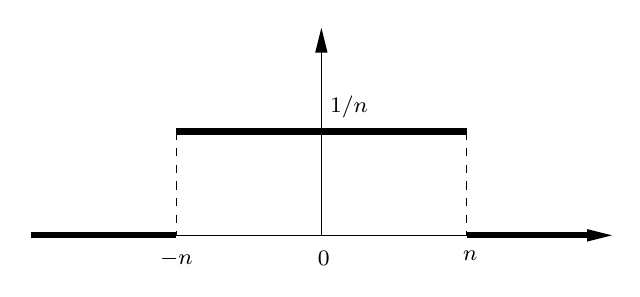
\begin{tikzpicture}[x=0.75pt,y=0.75pt,yscale=-1,xscale=1]
		%uncomment if require: \path (0,257); %set diagram left start at 0, and has height of 257

		\draw (80,170) -- (358,170) ;
		\draw [shift={(360,170)}, rotate = 180] [fill={rgb, 255:red, 0; green, 0; blue, 0 }  ][line width=0.08]  [draw opacity=0] (12,-3) -- (0,0) -- (12,3) -- cycle;
		\draw (220,170) -- (220,72) ;
		\draw [shift={(220,70)}, rotate = 90] [fill={rgb, 255:red, 0; green, 0; blue, 0 }  ][line width=0.08]  [draw opacity=0] (12,-3) -- (0,0) -- (12,3) -- cycle;
		\draw [line width=2.25](150,120) -- (290,120) ;
		\draw  [dashed, very thin]  (290,120) -- (290,170) ;
		\draw  [dashed, very thin]  (150,120) -- (150,170) ;
		\draw [line width=2.25](80,170) -- (150,170) ;
		\draw [line width=2.25](290,170) -- (350,170) ;

		\draw (287,176.4) node [anchor=north west][inner sep=0.75pt]  [font=\footnotesize]  {$n$};
		\draw (223,101.4) node [anchor=north west][inner sep=0.75pt]  [font=\footnotesize]  {$1/n$};
		\draw (141,176.4) node [anchor=north west][inner sep=0.75pt]  [font=\footnotesize]  {$-n$};
		\draw (217,176.4) node [anchor=north west][inner sep=0.75pt]  [font=\footnotesize]  {$0$};
		\end{tikzpicture}
		\caption{Plot of the function of example \vref{ex:strict-fatou}.}
	\end{figure}
	\FloatBarrier
	Then the $\liminf\limits_{n \to + \infty} f_n(t) = 0$ for all $t \in \RR$ but $\int_\RR f_n \de \lambda = 2 > 0 \quad \forall n \in \NN_0$.
\end{exam}


\begin{proof}
	Set $g_n(t) = \inf_{j\geq n}f_j(t)$. So $g_n$ is measurable and $g_{n+1}\geq g_n$ in $\Omega$.\\
	By definition of inferior limit we have:
	$$ \sup_{n\in \NN}g_n = \liminf_{n\to \infty} f_n.$$
	Using the monotone convergence theorem we get:
	$$\lim\limits_{n\to +\infty} \int_\Omega g_n\de \mu 
	= \int_\Omega \lim\limits_{n \to + \infty} g_n \de \mu 
	=\int_\Omega \liminf\limits_{n \to + \infty} f_n \de \mu$$
	By integral's monotonicity we obtain:
	$$\int_\Omega g_n \de\mu 
	\leq \int_\Omega f_n \de\mu;$$
	and considering the previous point we have:
	$$\lim\limits_{n \to + \infty}\int_\Omega g_n \de \mu \leq \liminf_{n \to + \infty} \int_\Omega f_n \de \mu$$
	which prove the thesis.
\end{proof}


